\documentclass{report}
\usepackage[utf8]{inputenc}
\usepackage{amsmath}
\usepackage{graphicx}
\usepackage[margin=1.5in]{geometry}

\title{Algoritmer og Datastrukturer Eksamen}
\author{Eksamensnummer: 137}
\date{\today}

\begin{document}
\maketitle

% ############################# OPGAVE 1 ####################################

\section*{Opgave 1}
\subsection*{Del 1.1}
En Fibonacci heap, $H$, er en mængde af rodfæstede træer der overholder \textit{min-heap property}'en - at nøglen i en knude er større eller lig med forældrens nøgle, hvilket resulterer i, at én af knuderne har den mindste nøgle med den mindste værdi i hele heap'en - den såkaldte  \textit{minimum node}. Vi tilgår en Fibonnaci heap med pointer'en \textit{H.min}, der pejer til denne  \textit{minimum node}. Træernes rødder har pejerene \textit{left} og \textit{right} der henholdsvis pejer til rødderne for træerne til højre og venstre for sig selv - dette skaber den såkaldte \textit{root list}. \\
Alle knuder har en pejer, \textit{p}, til sin forældre og en pejer, \textit{child}, til ét af sine børn; børnene er sammensat i en \textit{circular, doubly linked list}, hvilket herved gør det muligt for forældren at tilgå enhver af sine børn. Alle børn har pejerne \textit{left} og \textit{right}, der ved hjælp af den \textit{circular, doubly linked list} pejer til barnets højre og venstre søskene. Herudover har alle knuder attributen \textit{degree}, der beskriver antallet af børn som knuden har. \\
Herudover har alle knuder attributen \textit{mark}, der indikerer om en knude har mistet et barn siden knuden selv var lavet til et barn af en anden knude - dog bliver rodknuder ikke markeret, hvis når den mister et barn. En knude bliver \textit{unmarked} når den bliver lavet til et barn af en anden knude (hvilket kan ske når den mister sit andet barn), samt når den bliver skabt. \\
Fibonnaci heaps er en meget effektiv datastruktur, idet størstedelen af operationerne i amortiseret køretid kører i konstant tid - de eneste operationer der ikke kører i konstant tid er \texttt{EXTRACT-MIN} og \texttt{DELETE}, der har køretiderne $O(\lg n)$ og $O(\lg n)$ amortiseret køretid. Herved egner datastruktureren sig godt til algoritmer der anvender datastrukturerens operationer mange gange - og særlig godt, hvis \texttt{EXTRACT-MIN} og \texttt{DELETE} ikke anvendes særlig mange gange. Dette ses eksempelvis fra pensum i Prims algoritme og i Dijkstras algoritme. \\
Ved brugen af binære heaps har Prims algoritme en køretid på $O(E \lg V)$. Anvender algoritmen dog Fibonnaci heaps istedet, får algoritmen en køretid på $O(E + V \lg V)$, hvilket er bedre end implementationen med binære heaps, hvis tilfældet er, at antallet af knuder er meget mindre end antallet af kanter. \\
Dijkstras køretid afhænger af hvordan \textit{min-priorty} køen bliver implementeret - implementeres den ved hjælp af Fibonnaci heaps, bliver køretiden $O(V \lg V + E)$ - meget bedre end andre implementationers køretid, som for eksempel $O(V^2)$. Dette skyldes, at algoritmen generelt kalder \texttt{DECREASE-KEY} mange flere gange, end algoritmen kalder \texttt{EXTRACT-MIN}.

\newpage

\subsection*{Del 1.2}
Jeg har følgende algoritme for \texttt{INCREMENT}:
\begin{verbatim}
INCREMENT(A):
    i = 0
    while (i < A.length and A[i] == 9):
        A[i] = 0
        i += 1
    if (i < A.length):
        A[i] += 1
\end{verbatim}
Algoritmen fungerer ved at iterere igennem array $A$ indtil der findes en indgang der ikke er lig 9 - alle indgange op til dette sættes til 0, idet at lægge 1 til 9 resulterer i 0. Herefter lægges der 1 til den første værdi der ikke er lig 9, idet der herved er tale om et \textit{carry over} fra det forrige ciffer.

\newpage

\subsection*{Del 1.3}
Worst-case for algoritmen er hvis algoritmen får givet et array, hvor alle indgange er 9, altså hvor $A[i] = 9$ for $i = 0, 1, ..., 9$. Herved er while-loop'et i linje 2 nødt til at itere igennem hele array'et, hvilket giver en køretid på $O(k)$. \\
Acconting metoden til at vise den amortiserede køretid for \texttt{INCREMENT} kan vises, ved at lade de amortiserede omkostninger for at sætte et ciffer til 1, til at koste 10 credits - 1 credit bruges til at lægge 1 til cifferet, hvorimod de 9 overskydende gemmes på cifferet, som bruges til at betale for de næste 9 gange der skal lægges 1 til dette ciffer. Herved vil ethvert tal der ikke er lig 0, have nok credit til at sættes til 0 og der er derved ingen omkostninger ved at sætte et ciffer til 0, idet vi kan bruge de restende credit der ligger på cifferen. \\
Hertil kan vi bestemme den amortiserede køretid; at lægge 1 til et ciffer, udover hvis dette ciffer giver 1, bliver betalt af det credit der ligger på cifferet. Algoritmen lægger højst 1 til ét ciffer, i linje 6, hvilket betyder, at de amortiserede omkostninger maksimalt kan koste 9 (hvis cifferet går fra 0 til 1). Antallet af ciffer med credit kan ikke være negativt, hvilket betyder, at credit'et aldrig vil være negativt. Herved, ved kald til $n$ kald til \texttt{INCREMENT}, er de amortiserede omkostninger lig $O(n)$.

\newpage

% ################################### OPGAVE 2 ############################

\section*{Opgave 2}
\subsection*{Del 2.1}
Dynamisk Programming minder meget om \textit{Divide-and-Conquer}, idet begge paradigmer løser et problem, ved at dele problemet op i delproblmmer, efterfulgt af at løse disse delproblemer og tilsidst at kombinere disse delproblemer. Modsat problemer i \textit{Divide-and-Conquer}, så overlapper delproblemerne. Dette ses eksempelvis ved beregning af et Fibonacci tal:
\begin{center}
    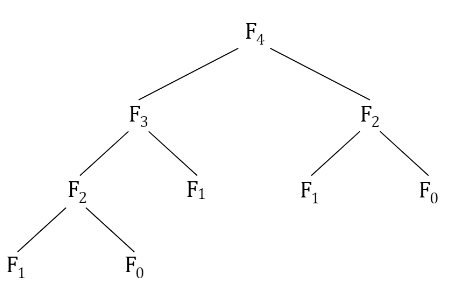
\includegraphics[height = 4 cm]{../entities/DP_fibonacci.PNG}
\end{center}
I dette eksempel er det tydeligt, at problemet består af overlappende delproblemer, idet Fibonacci-tallet $F_2$ skal udregnes 2 gange, for at udregne Fibonacci-tallet $F_4$. Ideen med Dynamisk Programmering er hertil at undgå at løse de overlappende delproblemer flere gange. \\
Ved Dynamisk Programmering er der to forskellige fremgangsmåder til, at løse et problem; \textit{top-down} og \textit{bottom-up}. \\
Ved \textit{top-down} løses problemerne rekursivt. Når et delproblem er løst, gemmes løsningen i hukommelsen og kan nemt slås op, hvis det samme delproblem er mødt igen senere. \\
Ved \textit{bottom-up} løses delproblemerne efter stigende størrelse efterfulgt af at gemme løsningen til disse delproblemer i hukommelsen. Herved, når et algoritmen støder på et nyt delproblem, er de delproblemer som den består af allerede løst. \\
Sammenlignes de to fremgangsmåder, så er det tydeligt, at de har sine fordele. \textit{top-down} har den fordel, at den kun løser den delproblemer der er nødvendige for de aktuelle problem - modsat \textit{bottom-up}, der løser alle delproblemer. På den anden side, så undgår \textit{top-down} rekursion, hvilket generelt resulterer i mindre konstantfaktorer i køretiden.

\newpage

\subsection*{Del 2.2}
Det er tydeligt, at rekursionsformlen er korrekt, idet den kører rekursivt igennem alle de mulige snit som der kan lægges på pladen og hertil finder ud af hvilke af disse snit der giver den største fortjeneste. Hertil finder rekursionsformlen altså den optimale løsning til alle de mulige delproblemer, som den finder ved at finde den optimale løsning til alle deldelproblemerne osv... Herved opnår problemet optimal delstruktur. \\
Hertil er det muligt at se, at $r_{b, h, s} = p_{b, h}$ når $b = h = 1$, idet det ikke er muligt at lægge et snit i pladen, så delpladerne har en heltalsbredde og heltalshøjde, samt $1 < b$ og $1 < h$. Det vil altså sige, at den eneste muligt i rekursionsformlen er, at returnere fortjenesten når der ikke skæres i pladen, altså, når $r_{b, h, s} = p_{b, h}$.

\end{document}